\documentclass[../mathNotesPreamble]{subfiles}

\begin{document}
%  \relscale{1.4} %TODO
  \section{2.4: Summarizing Categorical Distributions}
  \begin{defn*}
    \begin{itemize}
      \item The category that occurs most often is called the \textbf{mode} (similar to the usage with numerical variables).
      \item A distribution with a lot of \emph{diversity} is said to have a high \textbf{variability}.
    \end{itemize}
  \end{defn*}

  \emph{Note}: A categorical variable is considered bimodal \emph{only} if two categories are nearly tied for the mode.
  \vspace*{\baselineskip}

  \begin{ex*}
    Below are the results of a survey conducted in 2008, and again in 2012. How do the response compare?
  \end{ex*}

  \begin{center}
    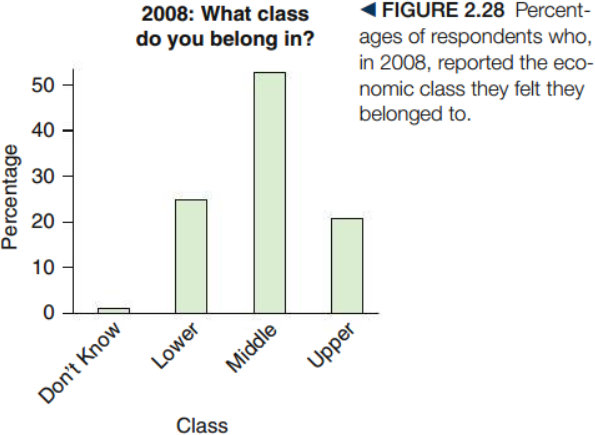
\includegraphics[width=0.425\linewidth]{images/math211_figure_2p28}
    \hspace*{\stretch{1}}
    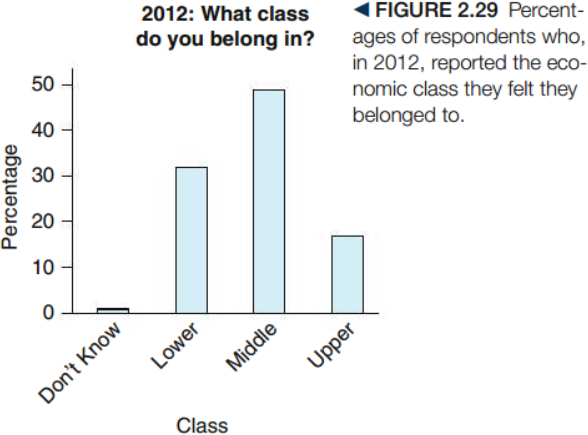
\includegraphics[width=0.425\linewidth]{images/math211_figure_2p29}
  \end{center}
  \vspace*{\stretch{1}}
  \pagebreak

  \begin{ex*}
    The ethnic composition of two schools in the Los Angeles City School System is presented in the bar charts below. Which school has the greater variability in ethnicity?
  \end{ex*}
  \begin{center}
    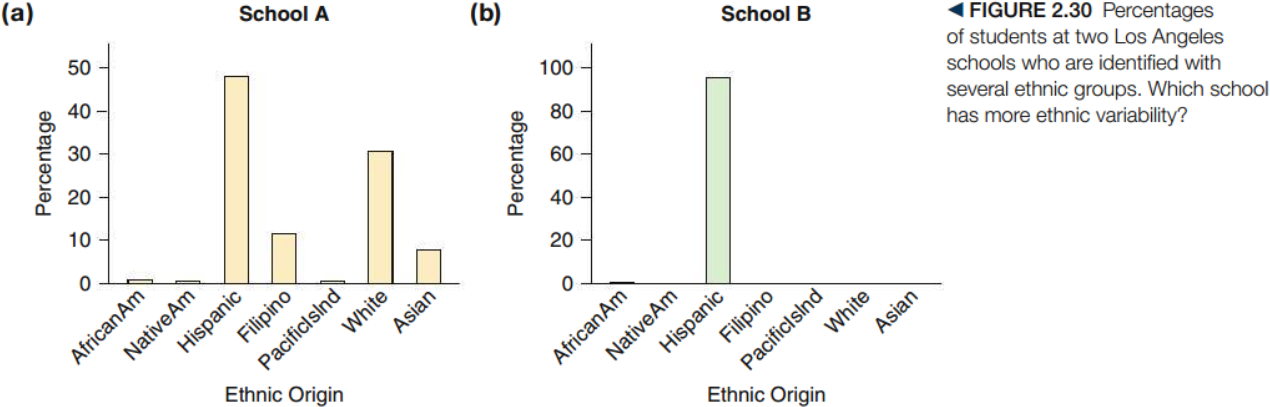
\includegraphics[width=0.975\linewidth]{images/math211_figure_2p30}
  \end{center}
  \pagebreak

  \begin{ex*}
    Compare the distributions below. What is the mode for each graph? Which graph demonstrates more variability?
  \end{ex*}
  \begin{center}
    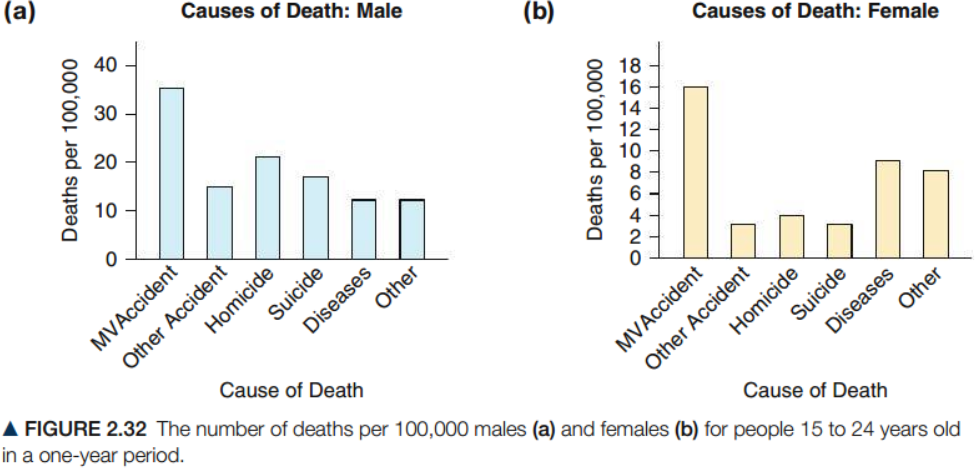
\includegraphics[width=0.975\linewidth]{images/math211_figure_2p32}
  \end{center}
  \vspace*{\stretch{1}}
  \begin{ex*}
    Compare the combined bar graphs below to the graphs above.
  \end{ex*}
  \begin{center}
    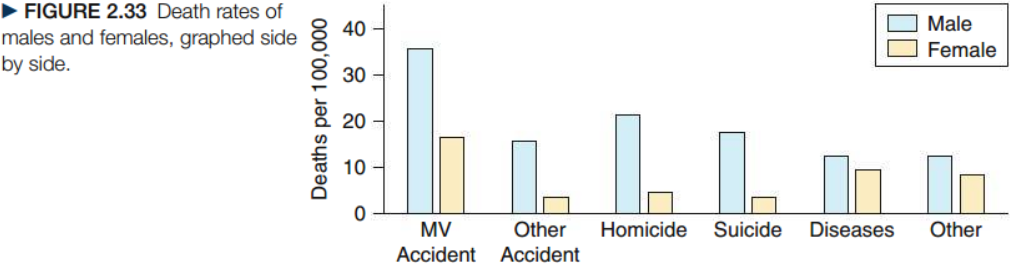
\includegraphics[width=0.9\linewidth]{images/math211_figure_2p33}
  \end{center}
  \vspace*{\stretch{1}}

  \pagebreak
\end{document}
